\subsection{User Interface}
\subsubsection{Hovedvindue}
I figur \ref{fig:gui} er et Mockup af GUI'en vist. I venstre side er der placeret en \textit{Start knap}, som skifter stadie til en \textit{Stop knap} når den er klikket. Under denne knap er en række indikatorer placeret til, at give operatøren feedback om status omkring initialiseringen af Hardwaren. 
I højre side af GUI'en er der placeret tekstfelter til, at give brugeren feedback omkring den nuværende sorteringscyklus, samt de anvendte indstillinger. Under disse felter er en knap til \textit{Indstillinger}. Når denne klikkes åbnes et nyt vindue, hvor operatøren kan ændre i indstillingerne. 
\begin{figure}[H]
	\centering
	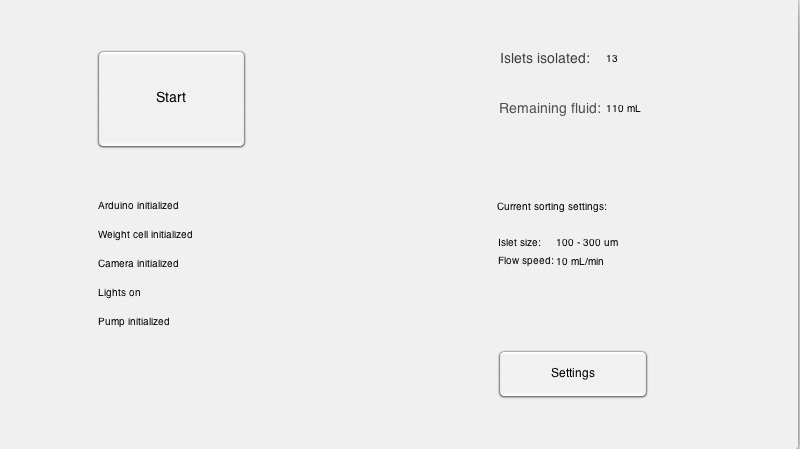
\includegraphics[width=1\textwidth]{billeder/GUI.png}
	\caption{Mockup af GUI}
	\label{fig:gui}
\end{figure}

\newpage
\subsubsection{Indstillinger}
I figur \ref{fig:gui_settings} er et Mockup af \textit{Indstillingsvinduet} vist. Via 2 tekstfelter har operatøren mulighed for, at ændre størrelsen for de celler som systemet skal sorterer. Herudover har operatøren via en dropdown menu mulighed for at ændre flowhastigheden for pumpen. I Indstillingsvinduet er der yderligere placeret en "Annuller" knap og en "Gem Indstillinger" knap.
\begin{figure}[H]
	\centering
	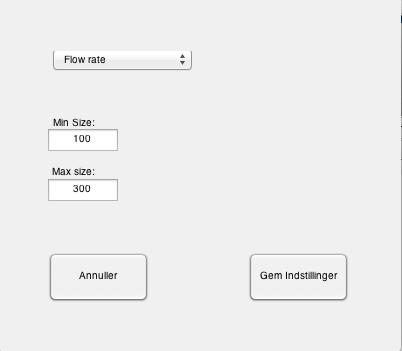
\includegraphics[width=0.5\textwidth]{billeder/GUI_settings.png}
	\caption{Mockup af Indstillinger}
	\label{fig:gui_settings}
\end{figure}


\newpage
\subsubsection{Callbacks}
For de 3 knapper i GUI'en oprettes der 3 callback funktioner, hvor forskellig kode eksekveres når knapperne klikkes. Disse 3 callback funktioner er nærmere beskrevet herunder bl.a. vha. flow chart diagrammer.
\subsubsection{Start Callback}
Denne callback funktion kaldes når operatøren klikker på Start knappen på GUI'en. Flowet i callbacket er vist i figur \ref{fig:act_start}.
\begin{figure}[H]
	\centering
	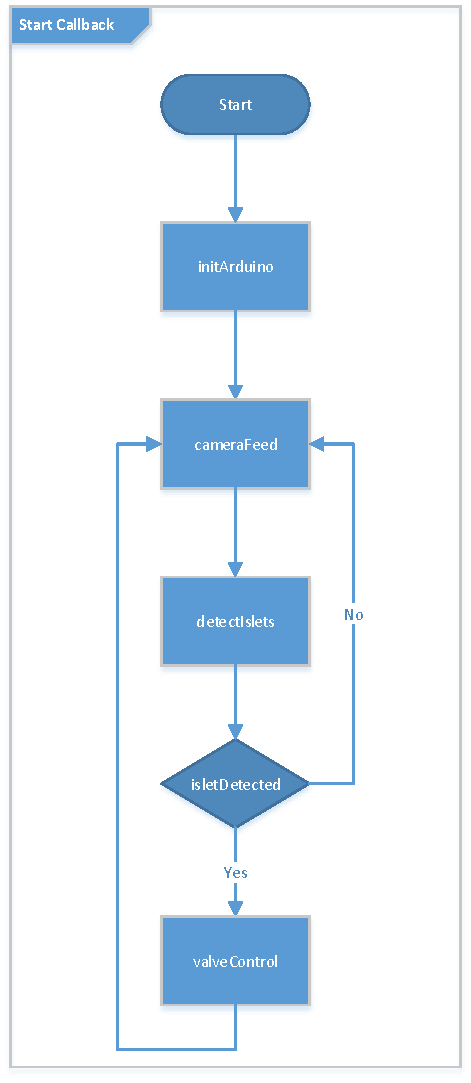
\includegraphics[width=0.5\textwidth]{billeder/act_start-crop.pdf}
	\caption{Flowchart diagram for Start Callback}
	\label{fig:act_start}
\end{figure}

\newpage
\subsubsection{Stop Callback}
Denne callback funktion kaldes når operatøren klikker på Stop knappen på GUI'en. Flowet i callbacket er vist i figur \ref{fig:act_stop}.
\begin{figure}[H]
	\centering
	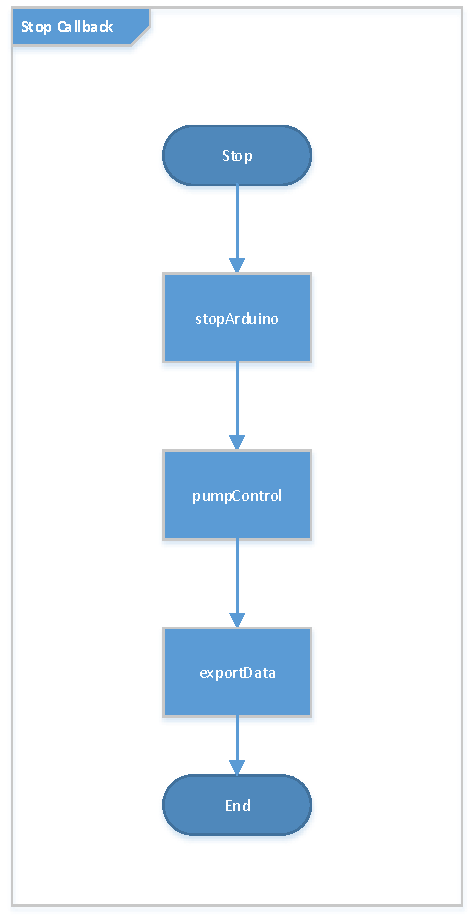
\includegraphics[width=0.5\textwidth]{billeder/act_stop-crop.pdf}
	\caption{Flowchart diagram for Stop Callback}
	\label{fig:act_stop}
\end{figure}

\newpage
\subsubsection{Indstillinger Callback}
Denne callback funktion kaldes når operatøren klikker på Settings knappen på GUI'en. Flowet i callbacket er vist i figur \ref{fig:act_settings}. Når knappen klikkes åbnes et nyt vindue, hvor systemets indstillinger kan ændres. De ændrede indstillinger anvendes i funktionerne detectIslets og pumpControl. 
\begin{figure}[H]
	\centering
	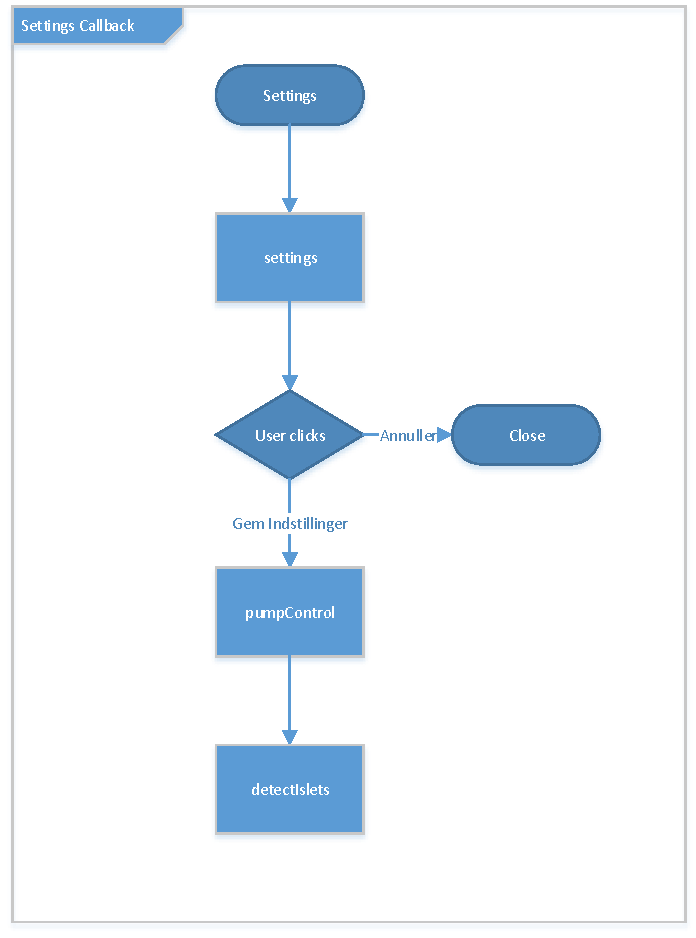
\includegraphics[width=0.5\textwidth]{billeder/act_settings-crop.pdf}
	\caption{Flowchart diagram for Settings Callback}
	\label{fig:act_settings}
\end{figure}
